Considera los dos triángulos que se muestran abajo en la Figura \ref{fig:20230323154518} (los triángulos no están dibujados a escala).

\begin{minipage}{0.6\textwidth}
    \textbf{¿Los dos triángulos son congruentes?}\\
    \emph{Escoge 1 respuesta:}\\

    \begin{choices}
        \choice Sí.
        \CorrectChoice No.
        \choice No hay suficiente información para decidir.
    \end{choices}
\end{minipage}%
\begin{minipage}{0.35\textwidth}
    \begin{figure}[H]
        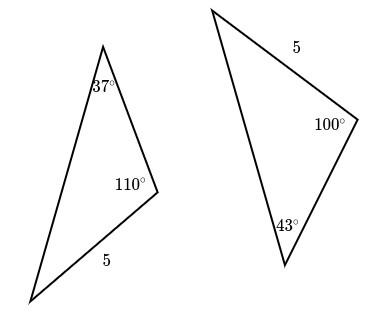
\includegraphics[width=\linewidth]{../images/20230323154518}
        \caption{}
        \label{fig:20230323154518}
    \end{figure}
\end{minipage}

\begin{solutionbox}{3cm}\footnotesize
    Dos triángulos son congruentes si tienen la misma forma y tamaño. En otras palabras, dos triángulos son congruentes si todos los lados y ángulos correspondientes son congruentes.

    Puesto que nos dan cuatro ángulos distintos, no hay manera de que los tres ángulos del primer triángulo sean congruentes a los ángulos del segundo triángulo.
    De hecho, como los ángulos de un triángulo suman 180$^\circ$, podemos calcular estos ángulos para verificarlo. Los ángulos del primer triángulo serían 45$^\circ$, 108$^\circ$ y 27$^\circ$, y los ángulos del segundo triángulo serían 73$^\circ$, 67$^\circ$ y 40$^\circ$.
    Los ángulos correspondientes no son congruentes. Por lo tanto los triángulos no pueden ser congruentes.

    \textbf{No, los triángulos no son congruentes.}
\end{solutionbox}